\protect\hyperlink{main-nav}{≡} \protect\hyperlink{close-nav}{×}

\hypertarget{section-2.4-product-and-quotient-rules}{%
\section{Section 2.4: Product and Quotient
Rules}\label{section-2.4-product-and-quotient-rules}}

The basic rules will let us tackle simple functions. But what happens if
we need the derivative of a combination of these functions?

\hypertarget{example-1}{%
\paragraph{Example 1}\label{example-1}}

Find the derivative of \textbackslash{}(
h(x)=\textbackslash{}left(4x\^{}3-11\textbackslash{}right)(x+3)
\textbackslash{})

This function is not a simple sum or difference of polynomials. It's a
product of polynomials. We can simply multiply it out to find its
derivative: \textbackslash{}{[} \textbackslash{}begin\{align*\} h(x)=\&
\textbackslash{}left(4x\^{}3-11\textbackslash{}right)(x+3)\textbackslash{}\textbackslash{}
=\& 4x\^{}4-11x+12x\^{}3-33\textbackslash{}\textbackslash{} h'(x)=\&
16x\^{}3-11+36x\^{}2 \textbackslash{}end\{align*\} \textbackslash{}{]}

Now suppose we wanted to find the derivative of
\textbackslash{}{[}f(x)=\textbackslash{}left(4x\^{}5+x\^{}3-1.5x\^{}2-11\textbackslash{}right)\textbackslash{}left(x\^{}7-7.25x\^{}5+120x+3\textbackslash{}right)\textbackslash{}{]}

This function is not a simple sum or difference of polynomials. It's a
product of polynomials. We could 'simply' multiply it out to find its
derivative as before -- who wants to volunteer? Nobody?

We'll need a rule for finding the derivative of a product so we don't
have to multiply everything out.

It would be great if we can just take the derivatives of the factors and
multiply them, but unfortunately that won't give the right answer. To
see that, consider finding derivative of \textbackslash{}(
h(x)=\textbackslash{}left(4x\^{}3-11\textbackslash{}right)(x+3)
\textbackslash{}). We already worked out the derivative, it is
\textbackslash{}( h'(x)=16x\^{}3-11+36x\^{}2 \textbackslash{}). What if
we try differentiating the factors and multiplying them? We'd get
\textbackslash{}(
h'(x)=\textbackslash{}left(12x\^{}2\textbackslash{}right)(1)=12x\^{}2
\textbackslash{}), which is radically different from the correct answer.

The rules for finding derivatives of products and quotients are a little
complicated, but they save us the much more complicated algebra we might
face if we were to try to multiply things out. They also let us deal
with products where the factors are not polynomials. We can use these
rules, together with the basic rules, to find derivatives of many
complicated looking functions.

To view this video please enable JavaScript, and consider upgrading to a
web browser that \href{http://videojs.com/html5-video-support/}{supports
HTML5 video}

To view this video please enable JavaScript, and consider upgrading to a
web browser that \href{http://videojs.com/html5-video-support/}{supports
HTML5 video}

\hypertarget{derivative-rules-product-and-quotient-rules}{%
\paragraph{Derivative Rules: Product and Quotient
Rules}\label{derivative-rules-product-and-quotient-rules}}

In what follows, \textbackslash{}(f\textbackslash{}) and
\textbackslash{}(g\textbackslash{}) are differentiable functions of
\textbackslash{}(x\textbackslash{}).

\hypertarget{product-rule}{%
\subparagraph{Product Rule}\label{product-rule}}

\textbackslash{}(\textbackslash{}frac\{d\}\{dx\}\textbackslash{}left(
f\textbackslash{}cdot g \textbackslash{}right)=f'\textbackslash{}cdot
g+f\textbackslash{}cdot g'\textbackslash{})

The derivative of the first factor times the second left alone, plus the
first left alone times the derivative of the second.

The product rule can extend to a product of several functions; the
pattern continues -- take the derivative of each factor in turn,
multiplied by all the other factors left alone, and add them up:
\textbackslash{}{[}\textbackslash{}frac\{d\}\{dx\}\textbackslash{}left(
f\textbackslash{}cdot g\textbackslash{}cdot h
\textbackslash{}right)=f'\textbackslash{}cdot g\textbackslash{}cdot
h+f\textbackslash{}cdot g'\textbackslash{}cdot h+f\textbackslash{}cdot
g\textbackslash{}cdot h'\textbackslash{}{]}

\hypertarget{quotient-rule}{%
\subparagraph{Quotient Rule}\label{quotient-rule}}

\textbackslash{}{[}\textbackslash{}frac\{d\}\{dx\}\textbackslash{}left(
\textbackslash{}frac\{f\}\{g\}
\textbackslash{}right)=\textbackslash{}frac\{f'\textbackslash{}cdot
g-f\textbackslash{}cdot g'\}\{g\^{}2\}\textbackslash{}{]}

The numerator of the result resembles the product rule, but there is a
minus instead of a plus; the minus sign goes with the
\textbackslash{}(g'\textbackslash{}). The denominator is simply the
square of the original denominator -- no derivatives there.

\hypertarget{example-2}{%
\paragraph{Example 2}\label{example-2}}

Find the derivative of \textbackslash{}(
h(x)=\textbackslash{}left(4x\^{}3-11\textbackslash{}right)(x+3)
\textbackslash{})

This is the same function we found the derivative of in Example 1, but
let's use the product rule and check to see if we get the same answer.
For this first example, we will provide a lot more detail and steps than
one usually actually shows when working a problem like this.

Notice we can think of \textbackslash{}(h(x)\textbackslash{}) as the
product of two functions \textbackslash{}( f(x)=4x\^{}3-11
\textbackslash{}) and \textbackslash{}( g(x)=x+3 \textbackslash{}).
Finding the derivative of each of these, \textbackslash{}{[}
f'(x)=12x\^{}2 \textbackslash{}
\textbackslash{}text\{and\}\textbackslash{} g'(x)=1. \textbackslash{}{]}

Using the product rule, \textbackslash{}{[}
\textbackslash{}begin\{align*\} h'(x)=\& (f')(g)+(f)(g')
\textbackslash{}\textbackslash{} =\&
\textbackslash{}left(12x\^{}2\textbackslash{}right)(x+3)+\textbackslash{}left(4x\^{}3-11\textbackslash{}right)(1)
\textbackslash{}end\{align*\} \textbackslash{}{]}

To check if this is equivalent to the answer we found in Example 1 we
could simplify: \textbackslash{}{[} \textbackslash{}begin\{align*\}
h'(x)=\&
\textbackslash{}left(12x\^{}2\textbackslash{}right)(x+3)+\textbackslash{}left(4x\^{}3-11\textbackslash{}right)(1)
\textbackslash{}\textbackslash{} =\& 12x\^{}3+36x\^{}2+4x\^{}3-11
\textbackslash{}\textbackslash{} =\& 16x\^{}3+36x\^{}2-11
\textbackslash{}end\{align*\} \textbackslash{}{]}

From this, we can see the answers are equivalent.

\hypertarget{example-3}{%
\paragraph{Example 3}\label{example-3}}

Find the derivative of \textbackslash{}(
F(t)=e\^{}t\textbackslash{}ln(t) \textbackslash{})

This is a product, so we need to use the product rule. I like to put
down empty parentheses to remind myself of the pattern; that way I don't
forget anything: \textbackslash{}{[}F'(t)=(\textbackslash{}
)(\textbackslash{} )+(\textbackslash{} )(\textbackslash{}
)\textbackslash{}{]}

Then I fill in the parentheses -- the first set gets the derivative of ,
the second gets left alone, the third gets left alone, and the fourth
gets the derivative of
\textbackslash{}{[}F'(t)=\textbackslash{}left(e\^{}t\textbackslash{}right)\textbackslash{}left(\textbackslash{}ln(t)\textbackslash{}right)+\textbackslash{}left(e\^{}t\textbackslash{}right)\textbackslash{}left(\textbackslash{}frac\{1\}\{t\}\textbackslash{}right)=e\^{}t\textbackslash{}ln(t)+\textbackslash{}frac\{e\^{}t\}\{t\}.\textbackslash{}{]}

Notice that this was one we could \emph{not} have done by ``multiplying
out.''

\hypertarget{example-4}{%
\paragraph{Example 4}\label{example-4}}

Find the derivative of \textbackslash{}(
y=\textbackslash{}frac\{x\^{}4+4\^{}x\}\{3+16x\^{}3\} \textbackslash{}).

This is a quotient, so we need to use the quotient rule. Again, you find
it helpful to put down the empty parentheses as a template:
\textbackslash{}{[}y'=\textbackslash{}frac\{(\textbackslash{}
)(\textbackslash{} )-(\textbackslash{} )(\textbackslash{}
)\}\{(\textbackslash{} )\^{}2\}\textbackslash{}{]}

Then fill in all the pieces:
\textbackslash{}{[}y'=\textbackslash{}frac\{\textbackslash{}left(4x\^{}3+\textbackslash{}ln(4)\textbackslash{}cdot
4\^{}x \textbackslash{}right)\textbackslash{}left(3+16x\^{}3
\textbackslash{}right)-\textbackslash{}left(x\^{}4+4\^{}x
\textbackslash{}right)\textbackslash{}left(48x\^{}2
\textbackslash{}right)\}\{\textbackslash{}left(3+16x\^{}3
\textbackslash{}right)\^{}2\}\textbackslash{}{]}

Now for goodness' sake don't try to simplify that! Remember that
``simple'' depends on what you will do next; in this case, we were asked
to find the derivative, and we've done that. I expect you to do any
``basic'' simplifications, such as multiplying constants together or
doing obvious cancellations or combining of terms, but otherwise please
STOP unless there is a reason to simplify further.

To view this video please enable JavaScript, and consider upgrading to a
web browser that \href{http://videojs.com/html5-video-support/}{supports
HTML5 video}

\hypertarget{example-5}{%
\paragraph{Example 5}\label{example-5}}

Suppose a large tank contains 8 kg of a chemical dissolved in 50 liters
of water. If a tap is opened and water is added to the tank at a rate of
5 liters per minute, at what rate is the concentration of chemical in
the tank changing after 4 minutes?

First we need to set up a model for the concentration of chemical. The
concentration would be measured as kg of chemical per liter of water,
kg/L. The number of kg of chemical stays constant at 8 kg, but the
quantity of water in the tank is increasing by 5 L/min. The total volume
of water in the tank after \textbackslash{}(t\textbackslash{}) minutes
is \textbackslash{}(50 + 5t\textbackslash{}), so the concentration after
\textbackslash{}(t\textbackslash{}) minutes is
\textbackslash{}{[}c(t)=\textbackslash{}frac\{8\}\{50+5t\}.\textbackslash{}{]}

To find the rate at which the concentration is changing, we need the
derivative: \textbackslash{}{[} \textbackslash{}begin\{align*\} c'(t)=\&
\textbackslash{}frac\{\textbackslash{}frac\{d\}\{dt\}(8)\textbackslash{}cdot(50+5t)-(8)\textbackslash{}cdot\textbackslash{}frac\{d\}\{dt\}(50+5t)\}\{(50+5t)\^{}2\}
\textbackslash{}\textbackslash{} =\&
\textbackslash{}frac\{(0)\textbackslash{}cdot(50+5t)-(8)(5)\}\{(50+5t)\^{}2\}
\textbackslash{}\textbackslash{} =\&
-\textbackslash{}frac\{40\}\{(50+5t)\^{}2\}
\textbackslash{}end\{align*\} \textbackslash{}{]}

At \textbackslash{}(t = 4\textbackslash{}), \textbackslash{}{[}
c'(4)=-\textbackslash{}frac\{40\}\{(50+5(4))\^{}2\}\textbackslash{}approx
-0.00816.\textbackslash{}{]}

Note that the units here are kg per liter, per minute, or
\textbackslash{}(
\textbackslash{}frac\{\textbackslash{}text\{kg/L\}\}\{\textbackslash{}text\{min\}\}
\textbackslash{}). In other words, this tells us that after 4 minutes,
the concentration of chemical is \emph{decreasing} by 0.00816 kg/L each
minute.

\hypertarget{more-graphical-interpretations-of-the-basic-business-math-terms}{%
\subsection{More Graphical Interpretations of the Basic Business Math
Terms}\label{more-graphical-interpretations-of-the-basic-business-math-terms}}

Returning to our discussion of business and economics topics, in
addition to total cost and marginal cost, we often also want to talk
about average cost or average revenue.

Recall from the previous section that the \textbf{Average Cost}
(\textbf{AC}) for \textbackslash{}(q\textbackslash{}) items is the total
cost divided by \textbackslash{}(q\textbackslash{}), or
\textbackslash{}(AC(q)=\textbackslash{}frac\{TC\}\{q\}\textbackslash{}).
You can also talk about the average fixed cost,
\textbackslash{}(\textbackslash{}frac\{FC\}\{q\}\textbackslash{}), or
the average variable cost,
\textbackslash{}(\textbackslash{}frac\{TVC\}\{q\}\textbackslash{}).

Also recall that the \textbf{Average Revenue} (\textbf{AR}) for
\textbackslash{}(q\textbackslash{}) items is the total revenue divided
by \textbackslash{}(q\textbackslash{}), or
\textbackslash{}(AR(q)=\textbackslash{}frac\{TR\}\{q\}\textbackslash{}).

We already know that we can find average rates of change by finding
slopes of secant lines. AC, AR, MC, and MR are all rates of change, and
we can find them with slopes, too.

\textbackslash{}(AC(q)\textbackslash{}) is the slope of a diagonal line,
from (0, 0) to \textbackslash{}((q, TC(q))\textbackslash{}).

\textbackslash{}(AR(q)\textbackslash{}) is the slope of the line from
(0, 0) to \textbackslash{}((q, TR(q))\textbackslash{}).

\begin{figure}
\centering
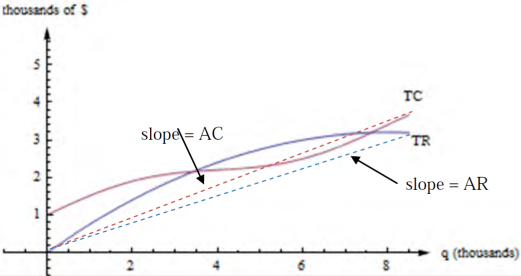
\includegraphics{images/image113.png}
\caption{}
\end{figure}

And just as we found marginal Total Cost, we can also find marginal
Average Cost.

\hypertarget{example-6}{%
\paragraph{Example 6}\label{example-6}}

The cost, in thousands of dollars, for producing
\textbackslash{}(x\textbackslash{}) thousand cellphone cases is given by
\textbackslash{}( C(x)=22+x-0.004x\^{}2 \textbackslash{}). Find

\begin{enumerate}
\tightlist
\item
  the Fixed Costs,
\item
  the Average Cost when 5 thousand, 10 thousand, or 20 thousand cases
  are produced,
\item
  the Marginal Average Cost when 5 thousand cases are produced.
\end{enumerate}

\begin{enumerate}
\item
  The fixed costs are the costs when no items are produced:
  \textbackslash{}( C(0)=22 \textbackslash{}) thousand dollars.
\item
  The average cost function is total cost divided by number of items, so
  \textbackslash{}{[}AC(x)=\textbackslash{}frac\{C(x)\}\{x\}=\textbackslash{}frac\{22+x-0.004x\^{}2\}\{x\}.
  \textbackslash{}{]}

  Note the units are thousands of dollars per thousands of items, which
  simplifies to just dollars per item.

  At a production of 5 thousand items: \textbackslash{}(
  AC(5)=\textbackslash{}frac\{22+5-0.004(5)\^{}2\}\{5\}=5.38
  \textbackslash{}) dollars per item.

  At a production of 10 thousand items: \textbackslash{}(
  AC(10)=\textbackslash{}frac\{22+5-0.004(10)\^{}2\}\{10\}=3.16
  \textbackslash{}) dollars per item.

  At a production of 20 thousand items: \textbackslash{}(
  AC(20)=\textbackslash{}frac\{22+5-0.004(20)\^{}2\}\{20\}=2.02
  \textbackslash{}) dollars per item.

  Notice that while the total cost increases with production, the
  average cost per item decreases, because the initial fixed costs are
  being distributed across more items.
\item
  For the marginal average cost, we need to find the derivative of the
  average cost function. We can either calculate this using the quotient
  rule, or we could use algebra to simplify the equation first (this is
  the easier option -- remember, simplifying before differentiating is
  almost always easier): \textbackslash{}{[}
  \textbackslash{}begin\{align*\} AC(x)=\&
  \textbackslash{}frac\{22+x-0.004x\^{}2\}\{x\}
  \textbackslash{}\textbackslash{} =\&
  \textbackslash{}frac\{22\}\{x\}+\textbackslash{}frac\{x\}\{x\}-\textbackslash{}frac\{0.004x\^{}2\}\{x\}
  \textbackslash{}\textbackslash{} =\&
  \textbackslash{}frac\{22\}\{x\}+1-0.004x
  \textbackslash{}\textbackslash{} =\& 22x\^{}\{-1\}+1-0.004x
  \textbackslash{}end\{align*\} \textbackslash{}{]} (Note: we haven't
  differentiated yet, only simplified.)

  Taking the derivative, \textbackslash{}{[}
  AC'(x)=-22x\^{}\{-2\}-0.004=-\textbackslash{}frac\{22\}\{x\^{}2\}-0.004.\textbackslash{}{]}

  When 5 thousand items are produced, \textbackslash{}{[}
  AC'(5)=-\textbackslash{}frac\{22\}\{5\^{}2\}-0.004=-0.884.\textbackslash{}{]}

  Since the units on \textbackslash{}(AC\textbackslash{}) are dollars
  per item, and the units on \textbackslash{}(x\textbackslash{}) are
  thousands of items, the units on \textbackslash{}(AC'\textbackslash{})
  are dollars per item per thousands of items. This tells us that when 5
  thousand items are produced, the average cost per item is
  \emph{decreasing} by \$0.884 for each additional thousand items
  produced.
\end{enumerate}

\begin{longtable}[]{@{}ll@{}}
\toprule
\endhead
\href{section2-3.php}{← Previous Section} & \href{section2-5.php}{Next
Section →}\tabularnewline
\bottomrule
\end{longtable}
